\chapter{内能~~能的转化和守恒定律}\label{chapter-internal-energy-and-laws-of-conversion-and-conservation-of-sssenergy}


\section{物体的内能}
\subsection{分子的动能~~温度}
既然组成物体的分子不停地做无规则运动,那么,像一切运动着的物体一样,做热运动的分子也具有动能.

物体里分子运动的速率是不同的,有的大,有的小,因此各个分子的动能并不相同.
在热现象的研究中,我们所关心的不是物体里每个分子的动能,而是所有分子的动能的平均值.这个平均值叫做分子热运动的平均动能.

温度升高,物体分子的热运动加剧,分子热运动的平均动能也增加.
温度越高,分子热运动的平均动能越大.
温度越低,分子热运动的平均动能越小.
从分子运动论的观点看来,\textit{温度是物体分子热运动的平均动能的标志}.这样,分子运动论使我们懂得了温度的微观含义.

\subsection{分子势能} 

分子间存在相互作用力,因此分子间具有由它们的相对位置决定的势能,这就是分子势能.

分子间的距离大于$r_0$(见图~\ref{fig_B_1-7})的时候,分子间的相互作用表现为引力,要增大分子间的距离必须克服引力做功,因此分子势能随着分子间的距离的增大而增大.这种情形同弹簧被拉长时弹性势能的变化相似.分子间的距离小于$r_0$的
时候,分子间的相互作用表现为斥力,要减小分子间的距离必须克服斥力做功,因此分子势能随着分子间的距离减小而增大.这种情形同弹簧被压缩时弹性势能的变化相似.

物体的体积发生变化时,分子间的距离也发生变化,因而分子势能随着发生变化.可见分子势能跟物体的体积有关系.

气体分子间的距离较大,分子的相互作用是引力.对气体来说,体积增大,分子间的距离增大,分子势能增加;体积缩小,分子间的距离减小,分子势能减少.

\subsection{物体的内能} 

物体中所有分子的热运动的动能和分子势能的总和,叫做物体的\textbf{内能}.一切物体都是由不停地做无规则热运动并且相互作用着的分子组成的,因此任何物体都具有内能.

由于分子热运动的平均动能跟温度有关系,分子势能跟体积有关系,因此物体的内能跟物体的温度和体积有关系.温度升高时,分子的动能增加,因而物体的内能增加.体积变化时,分子势能发生变化,因而物体的内能发生变化.

任何物体都具有内能,它同时还可以具有机械能.例如正在空中飞行的炮弹,除了具有内能,还具有机械能——动能和重力势能.下面我们要研究内能的变化,在作这种研究的时候,我们暂时不考虑作为研究对象的那个物体的机械能的变化.

顺便指出:我们过去常常提到热能,学过内能后应该知道,所谓热能不过是内能的一种通俗的说法.

\section*{阅读材料:热的本质}
热的本质是什么?为了弄清这个问题,人类经历了一段
曲折的认识过程.在二百多年以前,人们普遍认为热是一种特殊的物质——热质.
热质是一种没有质量的流质,它既不能产生,也不能消失,总保持守恒.
一个地方的热质多了,另一个地方的热质要变少.热质流入一个物体,物体含有的热质多了,温度就升高;热质从一个物体流出,物体含有的热质少了,温度就降低.这就是热质说.
热质说成功地说明了有关热传导和热量测定的一些实验事实,直到十九世纪初大多数学者都支持热质说.

热质说碰到的最大困难是对摩擦生热现象的解释.1798
年,本杰明$\cdot$汤普森(伦福德伯爵)在慕尼黑指导军工生产时发现:用钻头加工炮筒时,摩擦可以产生大量的热,使炮筒的温度升得很高,而且只要钻孔继续进行,就会不断地产生出大量的热来,好像物体里含有的热质是取之不尽的,热质并不守恒.
维护热质说的人解释说:炮筒温度升高,是由于钻下来的铜屑的比热减小了,铜屑放出的热质被炮筒所吸收.伦福德测定了钻下来的铜屑的比热,证明比热一点也没减小.伦福德的实验给热质说一个致命的打击.
伦福德从大量实验中得出结论:热不可能是一种物质,只能认为热是一种运动.

后来还有许多人研究了热和机械功的关系.
十九世纪中叶建立了能的转化和守恒定律,确认热是能的一种形式,它可以跟机械能、电能等相互转化,并在转化中守恒,而不存在守
恒的热质.能的转化和守恒定律的建立,彻底否定了热质说,同时为分子运动论的发展开辟了道路.而分子运动论进一步从微观上研究热现象,说明热现象是大量分子做无规则运动的表现,热这种形式的能是大量做无规则运动的分子具有的能,即课文中讲的内能.这样,人们对热的本质获得了正确认识.


\subsection*{练习一}
\begin{enumerate}
\item 壶里的水被加热而温度升高,水的内能怎样改变?液体的热膨胀很小,可不予考虑.
\item 一根烧红了的铁棍逐渐冷却下来,铁棍的内能怎样改变?固体的热膨胀很小,可不予考虑.
\item 容器里装着一定质量的气体,在保持体积不变的条件下使它的温度升高,气体的内能怎样改变?在保持温度不变的条件下把气体压缩,气体的内能怎样改变?
\item 设想我们对固体进行压缩.当分子间的距离小于$r_0$时,随着固体被压缩分子势能怎样改变?
\item 一颗炮弹在高空中以某一速度$v$飞行.
由于炮弹中所有分子都具有这一速度,所以分子具有动能.
又由于所有分子都在高处,所以分子具有势能.所有分子的上述动能和势能的总和就是炮弹的内能.上述说法正确不正确?为什么?
\end{enumerate}

\section{改变内能的两种方式}
在热学研究中所涉及的总是内能的变化.那么,什么物理过程可以改变物体的内能呢?

做功可以改变物体的内能.用锯条锯木头,我们克服摩
擦力做了功,锯条和木头的温度升高,内能增加.这类所谓摩擦生热的现象,是大家都知道的.物体在非弹性碰撞中做功,可以使它们的温度升高,内能增加.
用搅拌器在水中搅拌做功,可以使水的温度升高,内能增加.气体被压缩或膨胀时做功,气体的内能就发生变化.
在一个厚壁玻璃筒里放一块浸过
乙醚的棉花,迅速压下活塞对筒内空气做功,空气的内能增加,温度升高,达到乙醚的着火点,浸了乙醚的棉花就燃烧起来(图~\ref{fig_B_2-1}).柴油机就是利用这个道理来点火,使喷入气缸内的雾状柴油燃烧的.热机气缸内高温高压的气体膨胀时做功,气体的温度降低,内能减少.热机就是利用这个道理对外做功的.

\begin{figure}[htbp]
    \centering
    
\includegraphics{fig/B/2-1.pdf}
    \caption{压缩气体做功,气体内能增加.}\label{fig_B_2-1}
\end{figure}

但做功并不是改变物体内能的唯一方式.灼热的火炉使它上面和周围的物体温度升高,这些物体的内能增加.
火炉熄灭后,这些物体的温度降低,内能又减少.
在这样的过程中,物体的内能改变了,但是并没有做功.
这种没有做功而使物体内能改变的物理过程叫做\textbf{热传递}.

可见,\textit{能够改变物体内能的物理过程有两种:做功和热传递}.

做功使物体的内能发生变化的时候,内能的变化就用功的数值来量度.
外界对物体做多少功,物体的内能就增加多少;物体对外界做多少功,物体的内能就减少多少.

热传递使物体的内能发生变化的时候,内能的变化是用热量来量度的.外界传递给物体多少热量,或者说物体吸收了多少热量,物体的内能就增加多少;物体传递给外界多少热量,或者说物体放出了多少热量,物体的内能就减少多少.

一杯水可以用热传递的方式传给它一定的热量,使它从
某一温度升高到另一温度;也可以用做功的方式,比如用搅拌器在水中搅拌,使它升高同样的温度.两种方式不同,得到的结果却相同.
除非事先知道,我们将无法区别是哪种方式使这杯水的内能增加的.可见,做功和热传递对改变物体的内能是等效的.

\section{热功当量}
既然做功和热传递对改变物体的内能是等效的,功和热量都可以用来量度内能的变化,那么功和热量之间就应该有确定的数量关系.

我们在初中学过,热量的单位是卡路里(简称卡,$\UcalA$),使1克水的温度升高1$\Ucede$所需的热量就是1卡.如果功和热量之间有确定的数量关系,1卡的热量相当于多少焦耳的功?相当于单位热量的功的数值叫做\textbf{热功当量}.历史上第一个用实验来测定热功当量的人是英国物理学家焦耳.他用各种不同的方法测定了热功当量,下面我们介绍其中最著名的一种(图~\ref{fig_B_2-2}).

\begin{figure}[htbp]
    \centering
    \begin{subfigure}{0.4\linewidth}
        \centering
        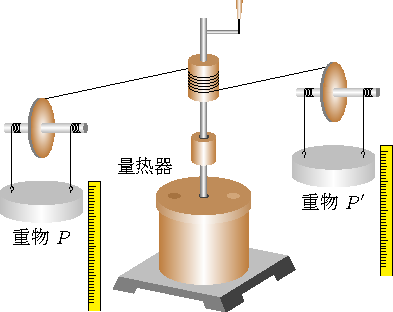
\includegraphics{fig/B/2-2a.pdf}
        \caption{}\label{fig_B_2-2a}
    \end{subfigure}
    \hfill
    \begin{subfigure}{0.4\linewidth}
        \centering
        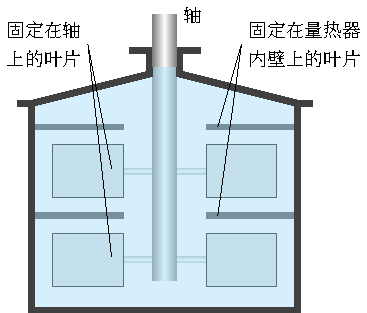
\includegraphics{fig/B/2-2b.pdf}
        \caption{}\label{fig_B_2-2b}
    \end{subfigure}
    \caption{左图是焦耳测定热功当量的装置;右图是量热器的纵截面图.}\label{fig_B_2-2}
\end{figure}


量热器里装着水,重物$P$和$P'$下落时带动量热器中的轴转动,轴上的叶片就带动周围的水随着转动.
量热器内壁上也固定着叶片,它们的作用是阻碍水的运动,增大摩擦.叶片搅动水做功,使水的内能增加,温度由$t_1$升高到$t_2$.已知每个重物的质量$M$和落下的高度$h$,我们可以算出这个功:
$$W=2Mgh $$
假定水的内能的增加不是由于做功而是由于热传递的结果,我们也可以算出使水的温度由$t_1$升高到$t_2$所需的热量:
\[Q=(m_1c_1+m_2c_2)(t_2-t_1)\]
其中$m_1$,$m_2$,$c_1$,$c_2$分别表示水和量热器的质量和比热.这样,就可以求出热功当量:
\[J=W/Q\]

这个实验焦耳做过多次,测得的热功当量的数值相同.他
又用水银代替水,重做上述实验,也得到相同的结果.
他还用其他方法来测定,结果仍然相同.焦耳同时代的和以后的许多科学家用不同的方法来测定,结果都相同.热功当量的数值通常可取为
\[ J=4.2 \UJcal \]

热功当量的数值的确定,证明功和热量之间存在着确定的数量关系,即$1 \Ucal =4.2 \UJ $,或者$1 \UJ=0.24 \Ucal$.
这进一步定量地证明做功和热传递对改变物体的内能是等效的.

热量的单位卡,是过去人们对热的本质认识不清楚的情况下规定的.既然功和热量之间有确定的数量关系,那么,功、热量和能量使用相同的单位,是很自然也很合理的.
现在,国际单位制中规定它们统一用焦耳作单位,并建议逐步取消卡这个单位.

\subsection*{练习二}
\begin{enumerate}
\item 举出几个实例来说明:做功可以改变物体的内能.
\item 锅炉中盛有150千克的水,由20$\Ucede$加热到100$\Ucede$,水的内能增加多少?
\item 一个物体的内能增加了20焦.如果物体跟周围环境不发生热交换,周围环境需要对物体做多少焦的功?如果周围环境对物体没有做功,需要传给物体多少焦的热量?
\item 设想在测定热功当量的不同实验中得到的结果并不相同,还能不能得到结论说:做功和热传递对改变物体的内能是等效的?讨论一下这个问题.
\item 在图~\ref{fig_B_2-2} 所示的实验中,已知重物$P$和$P'$的质量都是14千克,水的质量是7千克,重物连续从2米高处落下20次后,水的温度升高$0.37 \Ucede$.不考虑传给量热器和外界的热量,试根据这些数据计算热功当量.
\end{enumerate}



\section{能的转化和守恒定律}
\subsection{热力学第一定律} 

现在我们来研究功、热量跟内能变化之间的定量关系.

一个物体,如果它跟外界不发生热交换,也就是它既没有
吸收也没有放出热量,那么,外界对它做多少功,它的内能就增加多少.
设外界对物体所做的功为$W$,内能的增加为$\Delta E$,那么,$W=\Delta E$.在物体对外界做功的情况下,上式同样适用.这时$W$为负值,内能的增加$\Delta E$也是负值,表示内能减少.

如果外界既没有对物体做功,物体也没有对外界做功,那么物体吸收了多少热量,它的内能就增加多少.设物体吸收的热量为$Q$,内能的增加为$\Delta E$,那么,$Q=\Delta E$.在物体放出热量的情况下,上式同样适用,这时$Q$为负值,内能的增加$\Delta E$也是负值,表示内能减少.

在一般情况下,如果物体跟外界同时发生做功和热传递的过程,那么,外界对物体所做的功$W$加上物体从外界吸收的热量$Q$,等于物体内能的增加$\Delta E$.即
\[W+Q=\Delta E\]
上式所表示的功、热量跟内能变化之间的定量关系,在物理学中叫做\textbf{热力学第一定律}.

\subsection{能的转化和守恒定律} 
现在我们从能的转化的观点来考察热力学第一定律.我们知道,功是能的转化的量度,做功使内能发生变化时,其他形式的能和内能发生相互转化.在摩擦生热的现象中,克服摩擦力做多少功,就有多少机械能转
化成等量的内能.在图~\ref{fig_B_2-1} 所示的压缩气体做功的过程中,做多少功,就有多少机械能转化成等量的内能.气体膨胀做功的时候,做多少功,就有多少内能转化成等量的机械能.热传递使内能发生变化时,只是内能在物体之间的转移,而没有能量形式的转化.一个物体从外界吸收了多少热量,就有多少内能从外界转移给这个物体.这里我们看到,做功和热传递对改变物体的内能虽然等效,但从能的转化的观点来看却是有区别的.
热力学第一定律表示,做功和热传递提供给一个物体多少能量,物体的内能就增加多少,能量在转化或转移中守恒.

不但机械能,其他形式的能也可以和内能相互转化.通过电流的导线变热,电能转化成内能.燃料燃烧生热,化学能转化成内能.
炽热的灯丝发光,内能转化成光能.
实验证明,在这种转化中能量也守恒.

大量的事实证明:各种形式的能都可以相互转化,并且在转化中守恒.


\textbf{能量既不会凭空产生,也不会凭空消失,它只能从一种形式转化为别的形式,或者从一个物体转移到别的物体.}这就是\textbf{能的转化和守恒定律}.

现在我们利用这个定律来分析一下射到地球上的太阳能的转化.太阳把地面晒热,把空气晒热,把水面晒热并使一部分水蒸发.变热的空气上升,使空气流动而形成风,太阳能转化成空气的机械能.蒸发的水蒸气上升到空中形成云,以雨雪等形式落下来,通过江河流入海洋,太阳能转化成水的机械
能.太阳能的一部分被植物叶子吸收,发生光合作用,生成各
种有机化合物,太阳能转化成植物的化学能.植物作为食物被动物吃掉,植物的化学能转化成动物的化学能.人们以植物和动物为食物,从中获得了维持生命活动的能量.古代的植物和动物在地质变迁中转化成煤、石油、天然气,成为我们现代工农业生产的主要能源.
在水力发电站和火力发电站里,水的机械能,煤、石油和天然气的化学能转化成电能.
在工厂、农村和住宅中,电能通过各种电器转化成机械能、内能、光能等等.

物质有许多不同的运动形式,每种运动形式都有一种对应的能.跟机械运动对应的是机械能,跟热运动对应的是内能,跟其他运动形式对应的还有电能、磁能、化学能、原子能等等.能的不断转化表现了物质的运动不断地由一种形式转化为另一种形式.
能的转化和守恒定律就是关于自然界的这种转化过程的一条普遍定律.

\subsection{永动机不可能制成} 
历史上有不少人希望设计一种机器,这种机器不消耗任何能量,却可以源源不断地对外做功.这种机器被称为永动机.虽然经过多次尝试,作了各种努力,但无一例外地归于失败.这种尝试的失败导致了能的转化和守恒定律的发现.而能的转化和守恒定律则明确指出:任何一部机器只能使能量从一种形式转化为另一种形式,要对外
界做功必须消耗能量,不消耗能量便无法对外界做功,因而永动机不可能制成.我们利用自然,必须遵循自然界的规律,违反这种规律,就要失败.制造永动机只能是一种永远无法实现的幻想.

\begin{example}
    一定量的气体从外界吸收热量$6.36\times 10^4$卡,
内能增加$4.25\times 10^5$焦.
气体对外界做了功,还是外界对气体做了功?做多少功?    
\end{example}

\begin{solution}
利用热力学第一定律的公式进行计算,$W$、$Q$和$\Delta E$要统
一用焦耳作单位.
\[Q=6.36\times 10^{4} \Ucal =2.66\times 10^5 \UJ \]
由于$W+Q=\Delta E$,所以
\[\begin{split}
W=\Delta E-Q&=4.25 \times 10^5 \UJ -2.66\times 10^5 \UJ \\
&=1.59\times 10^5 \UJ
\end{split} \]
$W$为正值,表示外界对气体做了$1.59\times 10^5$焦的功.
\end{solution}

\subsection*{练习三}
\begin{enumerate}
\item 做功和热传递对改变物体的内能虽然等效,但从能的转化的观点来看是有区别的.这种区别是什么?
\item 在图~\ref{fig_B_2-2} 所示的焦耳测定热功当量的实验中,什么其他形式的能转化成了水的内能?在历史上,热功当量的确定为建立能的转化和守恒定律提供了坚实的实验基础.你怎样理解这句话?讨论一下这个问题.
\item 用活塞压缩气缸里的空气,对空气做了900焦的功,同时气缸向外散热210焦.空气的内能改变了多少?
\item 空气压缩机在一次压缩中,活塞对空气做了$2\times 10^5$焦的功,同时空气的内能增加$1.5\times 10^5$焦.这时空气向外界传递的热量是多少?
\item 如果用$Q$表示物体吸收的热量,用$W$表示物体对外界所做的功,热力学第一定律也可以表达为下式:
\[Q=\Delta E+W\]
怎样解释这个表达式的物理意义?试根据课文中的表达式推
导出这个表达式.
\end{enumerate}

\section{能的转化和守恒定律的建立及其意义}
能的转化和守恒定律,是在工业革命的直接影响下,经过许多物理学家的长期探索,在十九世纪确立的.
对这一定律的发现有重大贡献的物理学家中,特别值得我们纪念的有英国物理学家焦耳($1818 \sim 1889$)、德国医生兼物理学家迈尔($1814 \sim 1878$)、德国物理学家亥姆霍兹($1824 \sim 1894$).

焦耳一生致力于实验研究,他从1840年起在将近四十年的时间里,做了四百多次实验,用各种不同的方法测定了热功当量,为能的转化和守恒定律的建立提供了坚实的实验基础.迈尔指出能的转化的广泛存在,是世界上首先阐述能的转化和守恒思想的人.
他还从理论上计算出热功当量的数值.
亥姆霍兹分析了不同形式的能的转化和守恒,并且把这个结果跟永动机不可能制成联系起来.
他在1847年的论文中对能的转化和守恒定律作了清晰而全面的论述,使这个定律为人
们广泛接受.恩格斯曾经把这一定律称为“伟大的运动基本定律”,并把这一定律和细胞学说、达尔文的生物进化论一起称为十九世纪自然科学的三大发现.

能的转化和守恒定律自从建立以来,就是人们认识自然和改造自然的有力武器.从物理、化学、生物到天文、地质,以及各种工程技术,这一定律都发挥了重要的作用.可以说,没有别的定律能像这一定律那样把如此广泛的科学技术领域联
系起来,使不同领域的科学工作者具有一系列的共同语言.

人们利用能的转化和守恒定律来研究自然取得了许多重
大的成就.
下面我们简单介绍一个近代物理学研究中的例子.在三十年代初期,人们发现在某些原子核反应中能量似乎并不守恒,一部分能量消失了.当时一些人就认为这些实验事实表明能量并不是普遍守恒的.但是另一些人认为在这里能量也是守恒的,奥地利物理学家泡利($1900 \sim 1958$)在1933年提出,可能存在着一种当时并不知道的极其微小的粒子,所谓消失了的能量,就是被它们带走了.
后来意大利物理学家费密($1901 \sim 1954$)把这种粒子叫做中微子,并且发展了有关中微子的理论,认为它是一种不带电的、质量极其微小的粒子.以后人们一面继续从理论上研究这种假设的中微子,一面想办法用实验来探测中微子的存在.
直到1956年,在人们已经拥有核反应堆后,才在实验中证实了中微子是的确存在的.
这样,能的转化和守恒定律就直接导致了中微子的发现.

我们正在为实现我国的工业、农业、国防和科学技术的现代化而斗争.
在这一伟大事业中,能的转化和守恒定律将是我们手中的强有力的武器之一.

\section{能源的利用和开发}
机器的运转,金属的冶炼,火车的行驶,飞机的飞行,都需要能量.日常生活中做饭、取暖、照明等,也需要能量.
凡是能够提供能量的东西,都可以叫做能源.煤、石油、天然气在燃烧时可以提供能量,它们是能源.水力和风力可以提供能
量,它们也是能源.
能源是提高人民生活水平和进行社会主义现代化建设的重要物质基础.

人类在生产和生活中需要各种形式的能,其中用量最大的是内能、机械能和电能.我们可以按照需要把能源的能量转化成各种形式的能,以供应用.能源的利用过程,实质上是能的转化和传递的过程.

煤、石油、天然气等燃料,在各种各样的燃烧炉中燃烧,它们的化学能转化成内能.内能可以直接使用,以满足生产和生活的需要;也可以通过各种热机转化成机械能,然后再被使用.电能便于输送而且用起来方便,因此还可以用热机带动发电机进一步把能量转化成电能,这就是火力发电.

水力可以通过水轮机做功,风力可以通过风车做功,变为便于应用的机械能.还可以用水轮机或风车带动发电机进一步把能量转化成电能,这就是水力发电或风力发电.

能源的能量在转化中虽然保持守恒,但最后被有效利用的仅是其中的一部分.
因此,提高能源的利用率,有效地利用能源,是十分重要的.

燃料在燃烧炉中燃烧时,理论上虽然化学能可以全部转化成内能,实际上却只有一部分转化成可供利用的内能.原因是:燃烧不完全,一部分化学能没有发生转化,还有许多能量以散热的形式散失了.因此,要改进燃烧条件,促使燃料完全燃烧,并且要做好炉体、管道等设备的绝热保温,以减少热量的散失.

同燃料的化学能转化成内能相比,把内能转化成机械能要困难得多.从理论上讲,任何热机都不可能把内能全部转
化成机械能,一定要有一部分内能被废气所带走.
热机工作物质(蒸汽或燃气)的温度越高,内能转化成机械能的部分就越大.
因此,使用高温的蒸汽或燃气,是提高热机效率的有效途径.充分利用废气带走的内能,可以大幅度提高燃料的总利用率.
在火力发电站中,可以利用蒸汽轮机排出的蒸汽给工厂和居民供热,这就是电热并供的热电站.

电能便于输送,但是远距离输电按目前的技术水平能量损失也不小.各种用电设备的效率虽然比较高,但都有能量损失.
因此,提高电能输送和用电设备的效率也是节能的重要措施.

\begin{figure}[htbp]
    \centering
    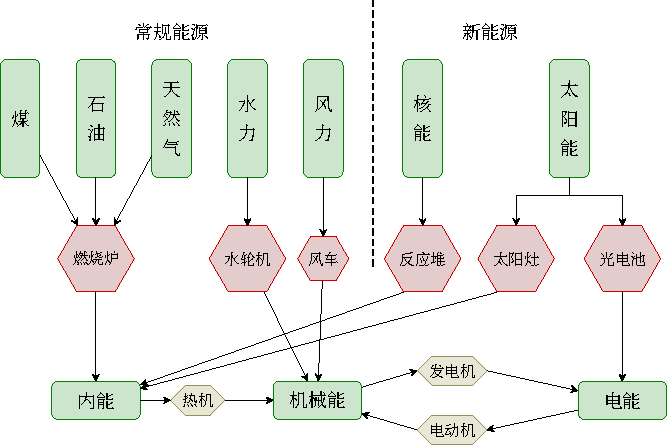
\includegraphics{fig/B/2-3.pdf}
    \caption{能源能量的转化和利用}\label{fig_B_2-3}
\end{figure}

现在人类社会使用的能源主要是煤、石油和天然气.但是煤、石油、天然气的储量是有限的,因此在合理开发和有效利用煤、石油、天然气等常规能源的同时,要不断探索能的转
化的新途径,大力开发和利用新能源.核能、太阳能、地热能、海洋能等都属于新能源.

核能也叫原子能,是原子核发生变化时释放出的能量.核能的发现虽然只有四十几年的历史,但是核能的利用已获得了巨大进展.原子核发生变化的方式有裂变和聚变.这方面的知识我们将在高中三年级学习.
目前裂变技术已经成熟.核燃料的核能通过反应堆可以转化成内能,再通过热机和发电机可以转化成电能,这就是核电站.对相同质量的燃料来说,核能比化学能要大几百万倍.1千克铀裂变时释放的能量相当于2400吨标准煤燃烧时释放的能量.因此,兴建核电站在经济上是合算的.目前我们正在兴建大型的核电站.核聚变能的利用还处于研究阶段,一旦成功将使人类享有可供长期使用的能源.

我们讲过,煤、石油和天然气的化学能归根到底来自太阳能.
作为新能源的太阳能,是指直接利用射到地球上的太阳能.
利用太阳灶可以把太阳能转化成内能.利用光电池还可以把太阳能直接转化成电能.太阳能是取之不尽,用之不竭的,但是目前利用太阳能存在着成本高、效率低等问题,要想大规模利用还需要取得技术上的突破.

地热能和海洋能的利用,目前处于试验研究阶段,大规模利用需要解决一系列技术问题.

我国是一个能源资源比较丰富的国家.煤、石油、天然气的储量丰富,水力资源居世界第一.但我国的能源利用率较低,浪费较大,能源供应比较紧张.
我国正大力加强能源的科学研究,以掌握有关的先进科学技术,抓好能源的开发,开展
以节能为中心的技术改造.这样我们将能够逐步克服能源供应的紧张,有条件依靠自己的能源资源实现社会主义四个现代化.同学们要好好学习,将来在能源科学技术中可以大显身手.

\subsection*{练习四}

\begin{enumerate}
\item 试说明下列现象中能量是怎样转化的:
\begin{enumerate}
    \item 在水平公路上行驶的汽车,发动机熄火之后,速度越来越小,最后停止.
    \item 在阻尼振动中,单摆的振幅越来越小,最后停下来.
    \item 火药爆炸产生燃气,子弹在燃气的推动下从枪膛发射出去,射穿一块钢板,速度减小.
    \item 用柴油机带动发电机发电,供给电动水泵抽水,把水从低处抽到高处.
\end{enumerate}

\item 取一个不高的横截面积是$ 300 \Ucmq $的圆筒,筒内装水0.6千克,用来测量射到地面的太阳能.
在太阳光垂直照射2分钟后,水的温度升高了1$\Ucede$.计算在阳光直射下地球表面每平方厘米每分钟获得的能量.
\item 从20米高处落下的水,如果水的势能的20\%用来使水的温度升高,水落下后的温度升高多少摄氏度?
\item 用铁锤打击铁钉,设打击时有80\%的机械能转化为内能,其中50\%用来使铁钉的温度升高.打击20次后,铁钉的温度升高多少摄氏度?已知铁锤的质量为1.2千克,铁锤打击铁钉时的速度为10$\Ums$,铁钉的质量为40克,铁的比热为$5.0\times 10^2  \UJkgcede $.

\item 在光滑的桌面上放着一个木块,铅弹从水平方向射中木块,把木块打落在地面上,落地点与桌边的水平距离为0.4米.铅弹射中木块后留在木块中.设增加的内能有60\%使铅弹的温度升高,铅弹的温度升高多少摄氏度?已知桌面高为0.8米,木块的质量为2千克,铅弹的质量为10克,比热为$1.3\times 10^2 \UJkgcede $.取$g=10 \Umsq $.

\end{enumerate}

\section*{复习题}
\begin{enumerate}
\item 从分子运动论的观点看来,温度标志着什么?什么是分子的动能?什么是分子势能?什么是物体的内能?物体的内能跟什么有关系?
\item 改变物体的内能有哪两种方式?从能的转化的观点来看,它们有什么区别?
\item 什么是热功当量?热功当量的测定在物理学的发展中有什么重要意义?
\item 热力学第一定律的内容是什么?写出它的数学表达式.
\item 能的转化和守恒定律的内容是什么?这个定律有什么重要意义?
\end{enumerate}




